% Use only LaTeX2e, calling the article.cls class and 12-point type.

\documentclass[10pt,a4paper]{mjcs}
% Use times if you have the font installed; otherwise, comment out the
% following line.

\usepackage{times}
\usepackage{graphicx}

\usepackage[figurename=Fig.]{caption}
\captionsetup[figure]{labelsep=period}
\captionsetup[table]{labelsep=period}

% The preamble here sets up a lot of new/revised commands and
% environments.  It's annoying, but please do *not* try to strip these
% out into a separate .sty file (which could lead to the loss of some
% information when we convert the file to other formats).  Instead, keep
% them in the preamble of your main LaTeX source file.


% The following parameters seem to provide a reasonable page setup.

\topmargin -1.5cm
\oddsidemargin 0.2cm
\textwidth 16cm
\textheight 24cm
%\footskip 1.0cm


\setlength{\parindent}{0em}
\setlength{\parskip}{0.7em}


%The next command sets up an environment for the abstract to your paper.

\newenvironment{mjcsabstract}{%
\begin{flushleft}
\textbf{\textit{ABSTRACT}}
\end{flushleft}

\it}


% If your reference list includes text notes as well as references,
% include the following line; otherwise, comment it out.

% Include your paper's title here

\title{Guidelines for Malaysian Journal of Computer Science}


% Place the author information here.  Please hand-code the contact
% information and notecalls; do *not* use \footnote commands.  Let the
% author contact information appear immediately below the author names
% as shown.  We would also prefer that you don't change the type-size
% settings shown here.

\author
{John Smith,$^{1\ast}$ Jane Doe,$^{1}$ Joe Scientist$^{2}$\\
\\
\normalsize{$^{1}$Department of Chemistry, University of Wherever,}\\
%\normalsize{An Unknown Address, Wherever, ST 00000, ABCD}\\
%\normalsize{$^{2}$Another Unknown Address, Palookaville, ST 99999, UBCD}\\
%\\
\normalsize{$^\ast$E-mail:  jsmith@wherever.edu.}
}

% Include the date command, but leave its argument blank.

\date{}


\usepackage{fancyhdr}

\pagestyle{fancy}
\fancyhf{}
\renewcommand{\headrulewidth}{0pt}
\rhead{Guidelines for Malaysian Journal of Computer Science}
%\lhead{Authors}



%%%%%%%%%%%%%%%%% END OF PREAMBLE %%%%%%%%%%%%%%%%



\begin{document}

% Double-space the manuscript.

\baselineskip12pt

% Make the title.

\maketitle



% Place your abstract within the special {sciabstract} environment.

\begin{mjcsabstract}
We accept submission of papers throughout the year. The accepted paper will be published in the next issue. Please submit your copy online or e-mail your submission softcopy (word document file) to editormjcs@um.edu.my with name(s), affiliation, contact person, address, email address included.
\end{mjcsabstract}

\keywords{MJCS, guidelines}


\section{Introduction}

The Malaysian Journal of Computer Science (MJCS) publishes original articles based on professional policies, practices, principles and progress in the field of information and communication technologies. Paper can be submitted to MJCS throughout the year, to the following email address: editormjcs@um.edu.my. Other modes of submissions will no longer be entertained.

Each submitted manuscript will be evaluated by one or more reviewer (s) on accuracy, originality of its technical/scientific contribution, quality and relevance. A manuscript may be accepted, returned for revision or rejected. The contact author of each paper will be notified of the result within 4 - 9 months of the submission date.

The reviewer(s) is (are) not responsible to edit poorly prepared papers. In order to avoid any embarrassment to authors, any undue burden for reviewers or editors, or any loss of time and effort, the authors are advised to engage competent colleagues to perform a thorough preliminary review before sending the papers to MJCS.

The author assumes full responsibility for the content of his/her article. He/she must ensure the accuracy of all data, statements and references. He/she also needs to ensure that the manuscript he/she submits to this journal is original and has never been published before.

Upon acceptance of the manuscript, the author is required to submit a camera-ready manuscript. A complimentary copy will be distributed to the author whose manuscript(s) is (are) published in this journal.

%\begin{figure}[htbp]
%\centering
%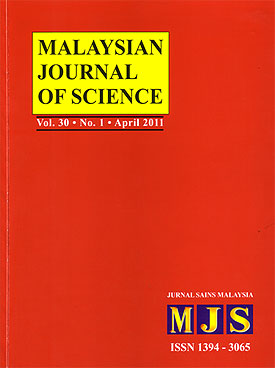
\includegraphics[scale=0.65]{cover_mjs.jpg}
%\caption{Malaysian Journal of Computer Science.}
%\label{mjcs}
%\end{figure}

\section{Style of Manuscript}
Manuscript must be written in English and prepared on A4-size paper with 3 cm, 2.5 cm, 2.5 cm and 2 cm margins from the top, bottom, left and right respectively. The manuscript must be prepared in Microsoft Word .doc format.

Centred at the top of the first page of a manuscript should be the complete title of the manuscript, full name(s) of author(s), affiliation(s), mailing and email address(es). This is followed by the abstract under the heading ABSTRACT (left-justified in italic, Times New Roman, 10 points), not exceeding 15 lines, keywords under the heading Keywords: (not more than eight keywords, in bold and italic, Times New Roman, 10 points) and followed by the text. The text should be typed and single-spaced, using a font similar to the one used in this text (Times New Roman, 10 points). Paragraphs should be separated by double spacing. The author(s) email address(es) are preferably official email address(es) associated with the affiliation(s).

A table or figure and the corresponding text should be placed on the same page. Otherwise it may be placed on the immediate following page. Its size should be smaller than the typed area.

A figure or photo should be labeled with “Fig.” and a table with “Table”. It must be assigned Arabic numerals as figure or table number; the figure number and caption should be placed below the figure, and the table number and caption should be placed on top of the table. The first letter of the caption should be in capital letter. Figures and tables should be placed in the middle of the page between left and right margins. Reference to the figure in the text should use “Fig.” instead of “Figure”.

\begin{table}[htbp]
\caption{Parameter values.}
\begin{center}
\begin{tabular}{|l|l|l|l|}
\hline
Parameters & $\alpha$ & $\beta$ & $\gamma$ \\
\hline
$\rho$ & 0 & 1 & 2 \\

$\gamma$ & 0.1 & 0.2 & 0.3 \\
\hline
\end{tabular}
\end{center}
\label{parameter_values}
\end{table}

Sections and subsections should be numbered and titled as 1.0, 2.0, etc. and 1.1, 1.2, 2.1,2.2.1, etc. respectively. Capital letters should be used for the section titles. For subsections, the first letter of each word should be in capital letter, followed by small letters.

Each manuscript should not exceed 20 pages including figures and tables. Do not paginate.

\subsection{References}
References should be noted with numbers \cite{01}, \cite{02}, \cite{03}, etc. at the right of the corresponding part of the text. The numbers should be the same as the references listed at the end of the manuscript under the heading REFERENCES (left-justified). Reference to articles in periodicals should take the form: initial(s) and name(s) of author(s), title (within quotes “ ”), title of journal (in italic), volume number, issue number, year published and page numbers.

Reference to conference proceedings/reports should take the form: initial(s) and name(s) of author(s), title (within quotes “ ”), name of conference in full (in italic), venue and date held, volume number (if any)/report number and page numbers. Reference to books should take the form: initial(s) and name(s) of author(s), title of book (in italic), edition (if any), place of publication, publisher and year published. Indicate chapters/page numbers where relevant.

The biography section should give the profiles of each author including name, academic achievements, affiliations to professional bodies, working experience, etc. within 100 words at the end of the manuscript. It should be placed below the references under the heading BIOGRAPHY (left-justified) and leaving a double spacing in between.

The Editor reserves the right to edit/format the manuscript to maintain a consistent style.

Please allow 4 -5 working days for receipt of acknowledgement.

\section*{Copyright}
It is a condition of publication that manuscripts submitted to the journal have not been published, accepted for publication, nor simultaneously submitted for publication elsewhere. By submitting a manuscript, the author(s) agree that copyright for the article is transferred to the publisher, if and when the manuscript is accepted for publication.

\begin{thebibliography}{10}

\bibitem{01}
L. Bernstein, {''Get The Design Right''}. IEEE Software, Vol. 10, No. 5, September 1993, pp. 61-63.

\bibitem{02}
Z. Razak, {''The Internet Global Villages''}, in Using IT to Build a Better Future Conference, Kuala Lumpur, 3 October 1995.

\bibitem{03}
J. Y. Halpern et al., {''Fault-Tolerant Clock Synchronisation''}, in Proceedings of the Third
Annual ACM Symposium: Principles of Distributed Computing, New York, ACM, 1984, pp.
89-102.

\end{thebibliography}

\end{document}




















